\documentclass[../main.tex]{subfiles}


\begin{document}

\section{Analyse}

%Indledning af analyse-afsnittet
\begin{flushleft} 
I analysefasen tages der brug af de påkrævet funktionelle og ikke-funktionelle krav til brætspillet, således at der kan oprettes et use case diagram samt en tabeloversigt over use-cases med ID-numre. 
Der vil blive udarbejdet use case beskrivelser udfra use case tabellen, hvor der henholdsvis vil gøres brug af detaljeret(fully-dressed) og brief form.
Ud fra use case beskrivelserne kan der hermed udarbejdes en domænemodel, som indeholder concepter af klasser.
En systemsekvensdiagram udarbejdes også da det er nødvendigt at få et dynamisk overblik over systemet for at kunne implementere koden for brætspillet.
\end{flushleft}


%Aktør
\subsection{Aktør}
Brætspillet indeholder én primær aktør:
\begin{itemize}
  \item  Spiller
\end{itemize}


%Use Case Diagram
\subsection{Use Case Diagram}
\begin{figure}[H]
    \centering
    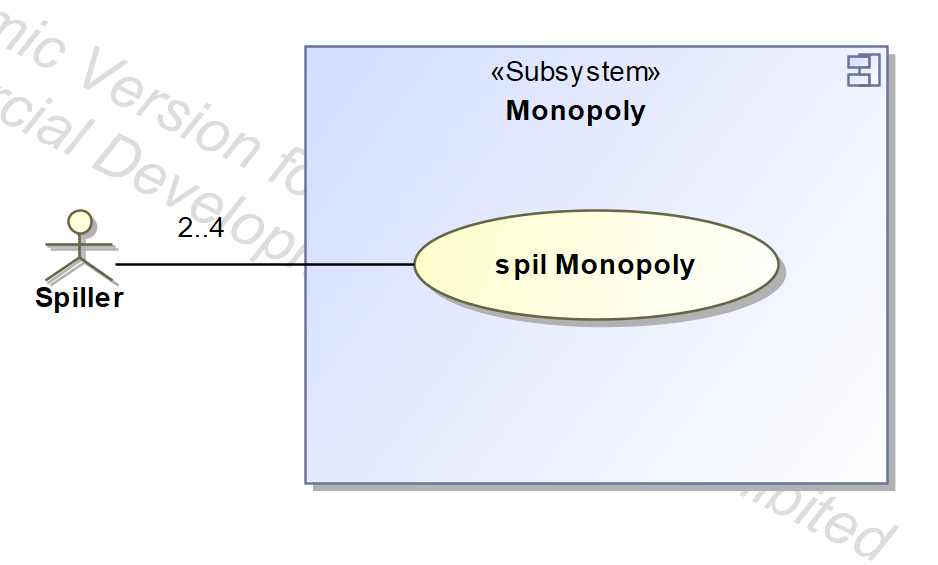
\includegraphics[width=0.6\linewidth]{figures/use-case_Diagram.png}
    \caption{Use-Case Diagram}
    \label{fig:UCDia}
\end{figure}

\newpage 

%Use Case tabel
\subsection{Use Case tabeloversigt}

%%%%%%%%%%%%%%%%%%%%%%%%%%%%%%%%%%
%Tabeloversigt for use case %%%%%%
\begin{table}[H]
\begin{tabular}{|c|l|p{0.5\linewidth}|}
\hline
 \textbf{ID} & \textbf{Funktion} & \textbf{Casual beskrivelse} \\\hline
\textbf{UC01} & Spil Monopoly  & 2-4 spillere spiller efter runde indtil der er fundet en vinder\\ \hline
\textbf{UC02} & Kast Terning   & En spiller kaster en terning og får givet en værdi i antal øjne på terningen \\ \hline
\textbf{UC03} & Ryk brik   & En spiller har kastet en terning og rykker til et nyt felt i urets retning\\ \hline
\textbf{UC04} & Passeret start   & En spiller lander eller har passeret start-feltet og modtager $\M$ penge\\ \hline
\textbf{UC05} & Lander på et ejendomsfelt  &  En spiller køber et felt og placerer et \textit{solgt}-skilt\\ \hline
\textbf{UC06} & Lander på Chance feltet   & En spiller tager et chancekort fra toppen af bunken, udfører en instruks og kortet lægges nederst i bunken igen.\\ \hline
\textbf{UC07} & Fængsel feltet   & En spiller lander på \textit{gå i fængsel}-feltet og rykker til \textit{fængsel}-feltet og kommer ud igen \\ \hline
\textbf{UC08} & Vind spil   & En spiller findes når en af spillerne er gået fallit  \\ \hline
\textbf{UC09} & (Gæld)   & (avanceret) \\ \hline
\end{tabular}
\caption{Use case tabeloversigt}
\label{tab:UC-tabeloversigt}
\end{table}


%%%%%%%%%%%%%%%%%%%%%%%%%%%%%%%%%%%%%%%%%
%Use cases og tilhørende beskrivelser %%%
\subsection{Use Case beskrivelser\textit{}}
\subsubsection{Detaljeret use-case beskrivelse:\textit{}}
%%%%%%%%%%%%%%%%%%%%%%%%%%%%%%%%%%%%%%%%%
%UC 05 - Ejendomsfelt %%%%%%%%%%%%%%%%%%%
\begin{table}[H]
    \begin{tabular}{|l|p{0.5\linewidth}|} 
    \hline 
    
\textbf{Use Case} & Lander på et ejendomsfelt  \\ \hline
\textbf{ID}                         & UC05     \\ \hline
\textbf{Scope}                      & \TODO... \\ \hline
\textbf{Level}                      & N/A      \\ \hline
\textbf{Primary actor}              & Spiller  \\ \hline
\textbf{Stakeholders and Interests} & N/A      \\ \hline
\textbf{Preconditions}             & At spilleren har påbegyndt brætspillet, det spillerens tur og spiller skal have rykket til et ejendomsfelt \\ \hline 
\textbf{Post condition}             & Spiller ejer enten  feltet, har betalt husleje eller gået fallit \\ \hline
\textbf{Main Success Scenario}      & \begin{tabular}[c]{@{}l@{}}1. Spiller rykker til ejendomsfelt \\ 2. Spiller køber feltet og betaler banken \\ 3. Spiller placerer et \textit{solgt}-skilt \\4. Spiller ejer nu feltet 
\end{tabular} \\ \hline
\textbf{Extensions (alternative flows)}  & \begin{tabular}[c]{@{}l@{}}
a. Hvis ingen ejer feltet  \\ \hspace{5mm} 
1. Hvis spiller ejer 12 ejendomme\\ \hspace{10mm}
1.1 \TODO?ingenting?\\ \hspace{5mm}
\vspace{2mm}
2. Spiller køber felt og placerer \textit{solgt}-skilt\\ 
b. Hvis spiller selv ejer feltet \\ \hspace{5mm} \vspace{2mm}
1. Ingenting sker\\ 
c. Hvis en anden spiller ejer feltet\\ \hspace{5mm}
1. Hvis en anden spiller ejer begge felter\\ \hspace{10mm} i samme farve\\ \hspace{10mm}
1.1 Spiller betaler dobbelt i husleje, \\\hspace{16mm} til den spiller som ejer ejendommen,\\\hspace{16mm} eller går fallit\\ \hspace{5mm}
2. Spiller betaler husleje, til den spiller \\\hspace{10mm} som ejer ejendommen, eller går fallit\\
d. Runden afsluttes 
\end{tabular} \\ \hline
\textbf{Special Requirements}             & N/A \\ \hline
\textbf{Technology and Data Variations List}     & N/A \\ \hline
\textbf{Frequency of Occurrence}                   & \begin{tabular}[c]{@{}l@{}}Der er høj frekvens, da brætspillet hoved-\\sagligt består i at købe og eje ejendomme
\end{tabular} \\ \hline
    \end{tabular}
    \caption{UC05 Lander på et ejendomsfelt}
    \label{tab:land_på_ejendomsfelt}
\end{table}


%%%%%%%%%%%%%%%%%%%%%%%%%%%%%%%%%%%%%%%%%
%UC 08 - Vind spil %%%%%%%%%%%%%%%%%
\begin{table}[H]
    \begin{tabular}{|l|p{0.52\linewidth}|} 
    \hline 
    
\textbf{Use Case} & Vind spil  \\ \hline
\textbf{ID}                         & UC08     \\ \hline
\textbf{Scope}                      & \TODO... \\ \hline
\textbf{Level}                      & N/A      \\ \hline
\textbf{Primary actor}              & Spiller  \\ \hline
\textbf{Stakeholders and Interests} & N/A      \\ \hline
\textbf{Preconditions}             & Der er en spiller, som er gået fallit. \\ \hline 
\textbf{Post condition}             & Der er fundet en vinder af spillet \\ \hline
\textbf{Main Success Scenario}      & \begin{tabular}[c]{@{}l@{}}1. En spiller går fallit \\ 2. Den spiller med flest penge vinder \\ 3. Spillet er afsluttet 
\end{tabular} \\ \hline
\textbf{Extensions (alternative flows)}  & \begin{tabular}[c]{@{}l@{}}
a. Hvis optælling er uafgjort   \\ \hspace{5mm} 
1. Læg værdi af ejendomme til optællingen\\ 
b. Den spiller med højst samlet værdi vinder \\
\end{tabular} \\ \hline
\textbf{Special Requirements}             & N/A \\ \hline
\textbf{Technology and Data Variations List}     & N/A \\ \hline
\textbf{Frequency of Occurrence}                   & \begin{tabular}[c]{@{}l@{}}Der er lav frekvens, da use case kun forekom-\\mer én gang i gennemspillet.
\end{tabular} \\ \hline
    \end{tabular}
    \caption{UC1 Spil Brætspil}
    \label{tab:vind_spil}
\end{table}


\subsubsection{Brief use-case beskrivelse:\textit{}}
%%%%%%%%%%%%%%
%SKABELON! %%%
%\begin{table}[H]
%\begin{tabular}{|l|p{0.75\linewidth}|}
%\hline
%\textbf{Use Case}       & Skabelon Brief \\ \hline
%\textbf{ID}                & X   \\ \hline
%\textbf{Brief Description} & ...   \\ \hline
%\textbf{Primary actors}    & ...   \\ \hline
%\textbf{Secondary actors}  & ...   \\ \hline
%\textbf{Preconditions}     & ...   \\ \hline
%\textbf{Main flow}         & 1.   \\ \hline
%\textbf{Post conditions}   & ...   \\ \hline
%\textbf{Alternative flows} & 1.   \\ \hline
%\end{tabular}
%\caption{skabelon}
%\label{tab:skabelon_brief}
%\end{table}

%%%%%%%%%%%%%%%%%%%%%%%%%%%%%%%%%%%%%%%%%
%UC 01 - SPIL MONOPOLY %%%%%%%%%%%%%%%%%%
\begin{table}[H]
\begin{tabular}{|l|p{0.75\linewidth}|}
\hline
\textbf{Use Case}          &    Spil Monopoly   \\ \hline
\textbf{ID}                &    UC01    \\ \hline
\textbf{Brief Description} &    2 til 4 spillere påbegynder brætspillet. Spillet spilles og der findes en vinder\\ \hline
\textbf{Primary actors}    &  Spiller  \\ \hline
\textbf{Secondary actors}  &    N/A \\ \hline
\textbf{Preconditions}     &    At man åbner Monopoly Junior spillet på sin computer\\ \hline
\textbf{Main flow}         &\begin{tabular}[c]{@{}l@{}}
1. Hver spiller indtaster sit navn og alder \\
2. Spillet spilles \\
3. Der findes en vinder \\
\end{tabular}\\ \hline
\textbf{Post conditions}   &    Der er fundet en vinder af spillet  \\ \hline
\textbf{Alternative flows} &    N/A \\ \hline
\end{tabular}
\caption{UC01 Spil Monopoly}
%\label{tab:spil_monopoly}
\end{table}

%%%%%%%%%%%%%%%%%%%%%%%%%%%%%%%%%%%%%%%%%
%UC 02 - KAST TERNING %%%%%%%%%%%%%%%%%%%
\begin{table}[H]
\begin{tabular}{|l|p{0.75\linewidth}|}
\hline
\textbf{Use Case}          & Kast terning      \\ \hline
\textbf{ID}                & UC02              \\ \hline
\textbf{Brief Description} & En spiller kaster en terning og får givet en værdi i antal øjne på terningen                                                \\ \hline
\textbf{Primary actors}    & Spiller          \\ \hline
\textbf{Secondary actors}  & N/A              \\ \hline
\textbf{Preconditions}     & At spilleren har påbegyndt brætspillet og det er spillers tur            \\ \hline
\textbf{Main flow}         & \begin{tabular}[c]{@{}l@{}}1. Når det er spillers tur kastes en terning \\ 2. Spiller kan aflæse antal øjne på terningen \\  
\end{tabular}                                  \\ \hline
\textbf{Post conditions}   & Spilleren rykkes det antal felter frem, som terningens værdi viser       \\ \hline
\textbf{Alternative flows} & N/A              \\ \hline
\end{tabular}
\caption{UC02 Kast terning}
%\label{tab:kast_terning}
\end{table}

%%%%%%%%%%%%%%%%%%%%%%%%%%%%%%%%%%%%%%%%%
%UC 03 - RYK BRIK %%%%%%%%%%%%%%%%%%%%%%%
\begin{table}[H]
\begin{tabular}{|l|p{0.75\linewidth}|}
\hline
\textbf{Use Case}          & Ryk brik          \\ \hline
\textbf{ID}                & UC03              \\ \hline
\textbf{Brief Description} & En spiller har kastet en terning og rykker til et nyt felt i urets retning                                                     \\ \hline
\textbf{Primary actors}    & Spiller.          \\ \hline
\textbf{Secondary actors}  & N/A               \\ \hline
\textbf{Preconditions}     & At spilleren har påbegyndt brætspillet og det er spillers tur            \\ \hline
\textbf{Main flow}         & \begin{tabular}[c]{@{}l@{}}1. Use case starter med spiller har slået med terningen. \\ 2. Spiller aflæser antal øjne på terningen \\ 3. Spiller rykker ternings værdi frem i felter (i urets retning) 
\end{tabular}                                  \\ \hline
\textbf{Post conditions}   & Spilleren er rykket til et nyt felt                                      \\ \hline
\textbf{Alternative flows} & 
\begin{tabular}[c]{@{}l@{}}1. Spiller rykker felt pga. konsekvens fra chancekort \\ 2. Spiller rykker til fængsel pga. \textit{Gå-I-Fængsel}-feltet
\end{tabular}                                  \\ \hline
\end{tabular}
\caption{UC03 Ryk brik}
%\label{tab:ryk_brik}
\end{table}

%%%%%%%%%%%%%%%%%%%%%%%%%%%%%%%%%%%%%%%%%
%UC 04 - PASSERET START %%%%%%%%%%%%%%%%%
\begin{table}[H]
\begin{tabular}{|l|p{0.75\linewidth}|}
\hline
\textbf{Use Case}          & Passeret start   \\ \hline
\textbf{ID}                & UC04              \\ \hline
\textbf{Brief Description} & En spiller lander eller har passeret \textit{Start}-feltet og modtager 2 $\M$     \\ \hline
\textbf{Primary actors}    & Spiller          \\ \hline
\textbf{Secondary actors}  & N/A              \\ \hline
\textbf{Preconditions}     & At spilleren har påbegyndt brætspillet, det er spillers tur og spiller har rykket til nyt felt                                  \\ \hline
\textbf{Main flow}         & \begin{tabular}[c]{@{}l@{}}1. Spiller rykker til nyt felt \\ 2. Spiller lander på eller passerer \textit{Start}-feltet  \\ 3. Spiller modtager 2 $\M$  
\end{tabular}                                  \\ \hline
\textbf{Post conditions}   & Spiller har modtaget 2 $\M$, hvis ikke spiller er i fængsel\\ \hline
\textbf{Alternative flows} &
\begin{tabular}[c]{@{}l@{}}1. Spiller rykker til fængsel pga. \textit{Gå-I-Fængsel}-feltet og modtager \\ ikke 2 $\M$ 
\end{tabular} 
\\ \hline
\end{tabular}
\caption{UC04 Passeret start}
%\label{tab:passeret_start}
\end{table}


%%%%%%%%%%%%%%%%%%%%%%%%%%%%%%%%%%%%%%%%%%% 
%UC 06 - Lander på chance %%%%%%%%%%%%%%%%%
\begin{table}[H]
\begin{tabular}{|l|p{0.75\linewidth}|}
\hline
\textbf{Use Case}          & Lander på \textit{Chance}-felt\\ \hline
\textbf{ID}                & UC06      \\ \hline
\textbf{Brief Description} & En spiller tager et chancekort fra toppen af bunken, udfører en instruks og kortet lægges nederst i bunken igen.\\ \hline
\textbf{Primary actors}    & Spiller\\ \hline
\textbf{Secondary actors}  & N/A \\ \hline
\textbf{Preconditions}     & At spilleren har påbegyndt sin tur og har landet på et \textit{chance}-felt  \\ \hline
\textbf{Main flow}         & \begin{tabular}[c]{@{}l@{}}1. Spiller har landtt på et \textit{chance}-felt  \\ 2. Spiller tager det øverste kort i chancekortbunken \\3. Spiller udfører instruks på kortet\\4. Spiller lægger det brugte kort nederst i bunken.
\end{tabular}                                  \\ \hline
\textbf{Post conditions}   & Spiller har trukket et chancekort, udført handling og lagt kort tilbage i bunken.      \\ \hline
\textbf{Alternative flows} & 
\begin{tabular}[c]{@{}l@{}} 1. Spiller har modtaget et \textit{Du løslades uden omkostninger}-kort \\ \hspace{5mm} 
1.1 Spiller gemmer kort til vedkommende er i fængsel\\
2. Spiller har givet et \textit{"Giv dette kort til.."}-kort til anden spiller\\\hspace{5mm} 
2.1 Den pågældende spiller, som har modtaget kortet, \\\hspace{10mm}gemmer kortet til det er vedkommendes tur\\
\end{tabular}
\\\hline
\end{tabular}
\caption{UC06 Lander på \textit{chance}-felt}
%\label{tab:chance_felt}
\end{table}


%%%%%%%%%%%%%%%%%%%%%%%%%%%%%%%%%
%UC07 Gå i fængsel %%%%%%%%%%%%%%
\begin{table}[H]
\begin{tabular}{|l|p{0.75\linewidth}|}
\hline
\textbf{Use Case}  &  Fængsel feltet  \\ \hline
\textbf{ID}  &  UC07 \\ \hline
\textbf{Brief Description} & Spilleren skal gå i fængsel og kommer ud igen \\ \hline
\textbf{Primary actors}    &  Spiller  \\ \hline
\textbf{Secondary actors}  & N/A  \\ \hline
\textbf{Preconditions}     &    At spilleren har kastet terningen og skal rykke til \textit{Gå-I-Fængsel}-feltet   \\ \hline
\textbf{Main flow} &   \begin{tabular}[c]{@{}l@{}}
     1. Use case starter med spiller har slået terningen\\
     2. Spilleren har slået det antal øjne hvor spilleren lander på\\
     \hspace{5mm} \textit{Gå-I-Fængsel}-feltet \\
     3. Spilleren skal nu flyttes til \textit{I-Fængsel}-feltet\\
     4. Spilleren skal nu ventet én runde\\
     5. Spilleren betaler 1 $\M$ for at komme ud af fængslet
\end{tabular}  \\ \hline
\textbf{Post conditions}   &  Spilleren kommer ud fængslet igen \\ \hline
\textbf{Alternative flows} & \begin{tabular}[c]{@{}l@{}}
1. Hvis spilleren har chancekortet \textit{Du løslades uden omkostninger} så\\ \hspace{5mm} må spilleren godt komme ud uden at skulle betale 1 $\M$ \\
2. Hvis spilleren ikke har nok penge til at betale for at komme ud\\
\hspace{5mm} går spilleren fallit
\end{tabular} \\\hline
\end{tabular}
\caption{UC07 Fængsel feltet}
%\label{tab:fængsel_felt}
\end{table}


%%%%%%%%%%%%%%%%%%%%%%%%%%%%%%%%%%%%%%%%%%%%%%%%
% Domænemodel %%%%%%%%%%%%%%%%%%%%%%%%%%%%%%%%%%
\subsection{Domænemodel}
\begin{figure}[H]
    \centering
    \includegraphics[width=0.7\linewidth]{figures/domæne-model.png}
    \caption{Domænemodel til spillet}
    \label{fig:domain}
\end{figure}


% Systemsekvensdiagram
\subsection{Systemsekvensdiagram}
\TODO
%\begin{figure}[H]
%    \centering
%    \includegraphics[width=0.7\linewidth]{figures/}
%    \caption{Systemsekvensdiagram}
%    \label{fig:systemsekvens}
%\end{figure}



\end{document}